\documentclass[a4paper,landscape,7pt,fleqn]{scrartcl}
\usepackage[english]{babel}
\usepackage[utf8]{inputenc}
\usepackage[dvips]{geometry}
\usepackage{latexsym}
\usepackage{multicol}
\usepackage{amsmath}
\usepackage{amsfonts}
\usepackage{amssymb}
\usepackage{array}
\usepackage{graphicx}
\usepackage{booktabs}
\usepackage{float} % add H as an option for floats
\usepackage{parskip}	% add no indentation to new paragraphs
\usepackage{empheq}		% emphasize (box) equations
\usepackage{enumitem} % description lists
\usepackage{fancyhdr}
\usepackage{lastpage}

\pagestyle{plain}
\typearea{16}
\columnsep 30pt
\columnseprule .4pt

\renewcommand*{\familydefault}{\sfdefault}		% set font to default sans-serif

\renewcommand{\labelitemi}{\tiny$\blacksquare$}		% change symbol of itemized lists

\renewcommand{\arraystretch}{1}
\renewcommand{\emph}[1]{\textbf{#1}}

\graphicspath{ {images/} }

\pagestyle{fancy}
\fancyhead{}
\setlength{\headheight}{0pt}
\setlength{\footheight}{14pt}
\renewcommand{\headrulewidth}{0pt}
\renewcommand{\footrulewidth}{0.5pt}
\lfoot{Fabian MARBACH}
\cfoot{p \thepage\ / \pageref{LastPage}}
\rfoot{Economic Foundations for Finance}

%\allowdisplaybreaks	% equations can be split on two pages/columns

\makeatletter
\renewcommand{\section}{\@startsection{section}{1}{0mm}%
{-2\baselineskip}{0.8\baselineskip}%
{\hrule depth 0.2pt width\columnwidth\hrule depth1.5pt
width0.25\columnwidth\vspace*{1.2em}\Large\bfseries}}
\makeatother

\makeatletter
\renewcommand{\subsection}{\@startsection{subsection}{1}{0mm}%
{-2\baselineskip}{0.8\baselineskip}%
{\hrule depth 0.2pt width\columnwidth\hrule depth0.75pt
width0.25\columnwidth\vspace*{1.2em}\large\bfseries}}
\makeatother

\makeatletter
\renewcommand{\subsubsection}{\@startsection{subsubsection}{1}{0mm}%
{-2\baselineskip}{0.8\baselineskip}%
{\hrule depth 0.2pt width\columnwidth\vspace*{1.2em}\normalsize\bfseries}}
\makeatother

\newcommand{\Mx}[1]{\begin{bmatrix}#1\end{bmatrix}}
\newcommand{\dd}[2]{\frac{\text{d}#1}{\text{d}#2}}
\newcommand{\DD}[2]{\frac{\text{D}#1}{\text{D}#2}}
\newcommand{\deidei}[2]{\frac{\partial#1}{\partial#2}}
\newcommand{\Lbrace}[1]{\left\{\begin{array}{ll}#1\end{array}\right.} % left brace with text

% Declare mathematical operators
\DeclareMathOperator{\erf}{erf}					% error function
\DeclareMathOperator{\Var}{Var}				% variance
\DeclareMathOperator{\Varn}{Varn}			% variation
\DeclareMathOperator{\QV}{QV}				% quadratic variation
\DeclareMathOperator{\Cov}{Cov}				% covariance
\DeclareMathOperator{\Bern}{Bern}			% Bernoulli distribution
\DeclareMathOperator{\Bin}{Bin}				% Binomial distribution
\DeclareMathOperator{\Geom}{Geom}		% Geometric distribution
\DeclareMathOperator{\Poisson}{Poisson}	% Poisson distribution
\DeclareMathOperator{\Gammaa}{Gamma}	% Gamma distribution
\DeclareMathOperator{\Adj}{Adj}				% Adjoint
\DeclareMathOperator{\argmax}{argmax}	% argmax


\begin{document}
\part*{Summary: Economic Foundations for Finance}
Fabian MARBACH, Autumn Semester 2015/16
\begin{multicols*}{3}
%\tableofcontents
%\end{multicols}
%{\vspace*{0.3cm}}
%{\hrule depth 0.2pt}
%{\vspace*{0.3cm}}
%\begin{multicols}{2}
\newpage
\raggedcolumns

\section{Game Theory}

\subsection{Basics}

\begin{itemize}
\item \emph{Players:} $\mathcal{I} = \lbrace 1,2,\ldots,I \rbrace$ \\
The players are usually assumed to act rationally.
\item \emph{Pure strategy:} $s_i \in S_i$ \\
Set of strategies available to player $i$: $S_i$ \\
Strategy set of the game: $S = S_1 \times S_2 \times \ldots \times S_i$ \\
Arbitrary element of the other players' strategies: $s_{-i} \in S_{-i}$
\item \emph{Mixed strategies:} $\sigma_i$ \\
i.e. $\sigma_i : S_i \to \mathbb{R}^+$ s.t. $\sum_{s_i \in S_i} \sigma_i(s_i) = 1$
\item \emph{Utility function:} $u_i : S \to \mathbb{R}$
\item \emph{Normal-form representation:} $G = \langle \mathcal{I},(S_i)_{i \in \mathcal{I}}, (u_i)_{i \in \mathcal{I}} \rangle$ \\
i.e. set of players $\mathcal{I}$, players' strategy spaces $S_1, \ldots, S_I$ and their utility functions $u_1, \ldots, u_I$
\item \emph{Extensive-form game:} set of players, course of the game (i.e. a tree of decision nodes), players' set of actions and information set at every node, payoff of all players at every terminal node
\item \emph{Rationality:} In general: rational players are aware of their available strategies $S_i$, form expectations about any unknowns, have clear preferences and choose their strategies according to utility maximization. \\
Rationality especially applies in case of imperfect information, incomplete information, mixed-strategies and about the reasoning of other players. \\
Playing a strategy $s_i$ is called rational for player $i$ iff $s_i$ is a best response given the belief of player $i$
\item \emph{Rationalizability:} The set of strategies that are rationally played when rationality of players is common knowledge. \\
\emph{Rationalizable strategies:} all strategies excluding never-best-response stragies
\item \emph{Subgame:} starts in a decision node that is a singleton information set, contains all subsequent successors of this node, and only these nodes, there are no broken information sets
\item \emph{Non-credible threats:} a threat of a player that is not in the interest of the player to be executed once the decision node has been reached
\item \emph{Pareto-optimum:} a state in which no player can be made better off without making another player worse off
\item \emph{Social optimum:} a state in which total utility is maximised
\end{itemize}

\subsection{Nash Equilibria (NE)}
\begin{itemize}
\item \emph{NE (in pure strategies):} each player knows knows the NE-strategy of the other players and no player has anything to gain by changing only his/her own strategy
\item \emph{NE in mixed strategies:} via indifference approach
\item \emph{Subgame-perfect Nash Equilibrium (SPNE):} In an extensive-form game $G$ a strategy profile $s^\ast$ is a SPNE if it is a NE of every subgame $G'$ of $G$ \\
Note that SPNE $\subseteq$ NE.
\end{itemize}

\subsection{Information}
\begin{itemize}
\item \emph{Information set:} a set of decision nodes at which the same player has to make a move but does not know which node of the information set has been reached
\item \emph{Perfect information:} an extensive-form game in which all information sets are singletons
\item \emph{Complete information:} an extensive-form game in which the extensive form is common knowledge
\item \emph{Incomplete information:} at least one player is uncertain about some player's payoff function
\end{itemize}

\subsection{Repeated games}
\begin{itemize}
\item \emph{Repeated games:} In a repeated game $G^T$ a finite, simultaneous-move \emph{stage game} $G$ is repeated $T$ times. \\
At each stage every player knows the actions of the previous stages and may condition his action on the history of actions.
\item \emph{Discount factor:} $\delta \in (0,1)$ \\
Frequent expressions:
\begin{align*}
\sum_{t=0}^\infty \delta^t = \frac{1}{1-\delta} \qquad \sum_{t=\tau}^\infty \delta^t = \frac{\delta^\tau}{1-\delta}
\end{align*}
\item \emph{Trigger strategy:} a strategy in which a player cooperates until someone fails to cooperate which triggers him to switch to noncooperation forever after.
\item \emph{Tit-for-Tat:} a strategy in which a player starts with cooperating and defects for one period everytime someone failed to cooperate but then switches back to cooperation again.
\item \emph{One-shot deviation principle:} a strategy set is a SPNE iff at every stage no player can profitably deviate by changing only his action at this stage.
\end{itemize}

\subsection{Bayesian games}
\begin{itemize}
\item \emph{Bayesian game:} finite set of players, finite action and type space for every player, beliefs of every player about the other players' types, payoff function of every player
\item \emph{Sequentially rational:} a player is sequentially rational if at every information set where it is his move his subsequent strategy is optimal wrt. his expected utility given his beliefs and the other player's strategies.
\item \emph{Consistent beliefs:} the probability for each node in an information set $H$ is determined by Bayes rule and the strategy profile $s$.
\end{itemize}

\emph{NE in Bayesian games:}

\begin{itemize}
\item \emph{Bayesian Nash Equilibrium (BNE):} a strategy profile $s$ and a belief assessment $q$ that maximize expected utility given player $i$'s beliefs for all players $i \in \mathcal{I}$ and for all types $\theta_i \in \Theta_i$.
\item \emph{Perfect Bayesian Equilibrium (PBE):} a strategy profile $s = (s_1, \ldots, s_I)$ and beliefs $q$ where the strategy profile $s$ is sequentially rational under $q$ and where the beliefs $q$ are consistent with strategy profile $s$.
\item \emph{Pooling equilibrium:} all types of a player behave the same
\item \emph{Separating equilibrium:} all types of a player behave differently
\item \emph{Semi-separating equilibrium:} some types choose the same action while other types choose another option
\end{itemize}

\newpage

\section{General Equilibrium Theory}

\subsection*{Structure}

\begin{itemize}
\item Financial markets and institutions
\item \emph{Basic economic model}
\item Extension of the model to \emph{capital}
\item Extension of the model to an \emph{infinite horizon}
\begin{itemize}
\item Extension of the model to \emph{uncertainty}
\item Extension of the model to \emph{exhaustible resources}
\end{itemize}
\end{itemize}

\subsection{Financial markets and institutions}

\paragraph{The three main functions of financial markets:}

\begin{itemize}
\item \emph{Intertemporal substitution of consumption:} Financial intermediaries enable individuals to distribute consumption as evenly as possible over time. \\
Usually, there is a positive interest rate. Thus, reducing consumption in one period is usually rewarded by increased consumption in a later period.
\item \emph{Risk diversification/sharing:} ''Wall street'' enables a more efficient risk sharing among many individuals than the mechanisms that belong solely to ''Main street''. \\
By purchasing a diversified stock portfolio, households are able to participate in the overall development of the ''Main street'' without incurring too large individual risks. \\
The returns on stocks are higher than the returns on bonds due to risk aversion (which follows from the principle of decreasing marginal utility), since stocks are procyclical (i.e. both stock prices and dividends) and since firms only take on debt if they expect to earn a higher return using this money within the firm.
\item \emph{Information aggregation:} In a sense, the stock market is a large polling institution which summarizes the opinion of many millions of people in share prices every day. \\
Markets are usually even better at providing estimations than rating agencies (e.g. compare credit spreads and ratings before the financial crisis of 2007-08).
\end{itemize}

\subsection{Production and utility function}

\paragraph{Consumption smoothing}

\begin{itemize}
\item \emph{Interest rate:} If $r>0$ then the interest rate may provide the consumer an incentive to postpone consumption. \\
The budget constraint can e.g. be written as:
\begin{align*}
C_0 + \frac{1}{1+r} C_1 \leq C_\text{max}
\end{align*}
\item \emph{Time preference:} $\beta > 0$ models the impatience of a consumer and thus may provide an incentive not to postpone consumption. \\
The utility function can e.g. be adjusted as:
\begin{align*}
\max\limits_{C_0,C_1} \sqrt{C_0} + \frac{1}{1+\beta} \sqrt{C_1}
\end{align*}
\item Consequently, impatience (i.e. time discounting) and positive interest rates have opposing effects.
\end{itemize}

\paragraph{Constant relative risk aversion (CRRA) utility}

\begin{align*}
U_t(C_t) = U(C_t) = \frac{C_t^{1-\gamma}}{1-\gamma}
\end{align*}

\subsection{Basic economic model}

\subsubsection{Production and utility function}

\paragraph{Production function}

Assumptions wrt. the production function $Y = F(L^d)$:
\begin{description}
\item{(F1)} No input, no output: $F(0) = 0$.
\item{(F2)} The more input, the more output: $F'(L^d) > 0$
\item{(F3)} Decreasing marginal productivity: $F''(F^d) > 0$
\end{description}

General production function: $F(L^d) = \left(L^d\right)^\gamma$, with $\gamma$ the output elasticity of labour.

Cobb-Douglas production function: $F(L^d) = \sqrt{L^d}$

\paragraph{Utility function}

Assumptions wrt. the utility function $U(C)$:
\begin{description}
\item{(U1)} The utility function is increasing in consumption: $U'(C) > 0$
\item{(U2)} The increase in utility function is decreasing in consumption: $U''(C) < 0$
\end{description}

\subsubsection{Market equilibrium}

\paragraph{Market equilibrium}

A market equilibrium is an allocation of supply and demand $(L^{s \ast}, Y^\ast, L^{d \ast}, C^\ast)$ as well as a price-wage system $(p^\ast, w^\ast)$, so that at those prices and wages the two agents, i.e. the firm and the household, can make no better choice, i.e. both decision problems are solved in an optimal manner. Furthermore, both goods and labour market clear.

\paragraph{Decision problem of the firm}

\begin{align*}
\max\limits_{L^d, Y} \underbrace{\pi}_\text{profit} &= \underbrace{p Y}_\text{total revenue} - \underbrace{w L^d}_\text{total cost} \\
\text{s.t. } \underbrace{Y}_\text{output} &= \underbrace{F(L^d)}_\text{production function}
\end{align*}

\paragraph{Decision problem of the household}

\begin{align*}
& \max\limits_{L^s, C} \underbrace{U(C)}_\text{utility} \\
\text{s.t. } & p C = \underbrace{w L^s}_\text{total wage} + \underbrace{\pi}_\text{profit} \qquad L^s \leq \underbrace{\bar L}_{\text{max } L^s}
\end{align*}

\paragraph{Market clearing}

\begin{align*}
L^{d \ast} = L^{s \ast} \quad , \quad C^\ast = Y^\ast
\end{align*}

\paragraph{Parameters}

{\setlength{\columnseprule}{0pt}
\begin{multicols}{2}
\begin{description}[style=multiline,leftmargin=0.6cm,font=\normalfont]
\item[$\pi$] profit
\item[$C$] consumption
\item[$Y$] output
\item[$U(\centerdot)$] utility function
\item[$F(\centerdot)$] production function
\item
\item[$w$] wage per unit of labour
\item[$p$] price per unit of output
\item[$L^d$] labour demand
\item[$L^s$] labour supply
\item[$\bar L$] maximum labour supply
\end{description}
\end{multicols}}

\subsubsection{Social planner's problem}

\begin{align*}
& \max\limits_{L, C} U(C) \\
\text{s.t. } & C = F(L), \qquad L \leq \bar L
\end{align*}

\subsubsection{Important properties of the market equilibrium}

\paragraph{First Welfare Theorem}

\begin{itemize}
\item The optimal solution from the perspective of the central planner can be achieved by two separate maximization problems (of the firm and the household) on the market.
\item The market equilibria are Pareto-efficient.
\end{itemize}

\paragraph{Walras Law (W)}

Labour market clears (i.e. $L^s = L^d$) $\iff$ Goods market clears (i.e. $C-Y$). \\
I.e. it holds $\forall p, w$:

\begin{align*}
p C &= w L^s + \pi = w L^s + p Y - w L^d \\
p \underbrace{(C-Y)}\limits_\text{goods market} &= w \underbrace{(L^s-L^d)}\limits_\text{labour market}
\end{align*}

\paragraph{Homogeneity property (H) / Absence of money illusion}

If $(p^\ast, w^\ast)$ is an equilibrium price system, then $\forall \lambda > 0$, $(\lambda p^\ast, \lambda w^\ast)$ is again an equilibrium price system, i.e. inflation has no impact on the market equilibrium.

Consequently, the real wage $\frac{w}{p}$ matters solely in equilibrium. \\
Hence the price $p$ can be normalized to $1$.

\paragraph{Stock prices, inflation and exchange rates}
\begin{itemize}
\item \emph{Stocks:} Value of the shares would equal the profit of the firms, i.e. $q = \pi$.
\item \emph{Inflation:} Nominal debt decreases with inflation in real terms. \\
In theory, real stock prices $q$ should be independent of the inflation rate $\lambda$ due to (H). \\
In fact, the real share value $q$ increases at moderate rates of inflation $\lambda$ since firms are also financed with debt.
However, at very high rates of inflation stock prices will fall since economies with such inflation rates do no longer work properly.
\item \emph{Exchange rate:} Due to (H), real stock prices do not depend on the value of the currency. Thus, changes in the exchange rate must be reflected in the nomial stock in local currency (e.g. DAX in EUR/CHF).
\end{itemize}

\subsubsection{Population growth and technological progress}

\paragraph{Technological progress}

\begin{itemize}
\item Rate of technological progress: $g > 0$
\item Production function: $F((1+g)L^d)$ \\
I.e. technological progress is labour-saving. Graphically, the production function is rotated upwards.
\item Effects of technological progress: \\
Labour remains constant. \\
Profit, output and wage increase. \\
Consumption p.c. increases.
\end{itemize}

\paragraph{Population growth}

\begin{itemize}
\item Rate of population growth: $n$
\item Amount of available labour: $\bar L_n = (1+n) \bar L_0$
\item Effects of population growth: \\
Labour, profit and output increase. \\
Wage decreases. \\
Consumption p.c. decreases.
\item Empirically, the returns on stocks tend to be higher in countries with high population growth.
\end{itemize}

\subsection{Extension of the model to capital}

\paragraph{Production function}

Assumptions wrt. the production function $Y = F(L^d,K^d)$:
\begin{description}
\item{(F1)} No input, no output: $F(0,K^d) = F(L^d,0) = 0$.
\item{(F2)} The more input, the more output: $\partial_L F(\centerdot) > 0, \partial_K F(\centerdot) > 0$
\item{(F3)} Decreasing marginal productivity: $\partial_L^2 F(\centerdot) < 0, \partial_K^2 F(\centerdot) < 0$
\item{(F4)} The margianl rate of substitution between capital and labour increases with labour:
\begin{align*}
\partial_L \left( -\frac{\partial_L F(\centerdot)}{\partial_K F(\centerdot)} \right) > 0
\end{align*}
\item{(F5)} Inada conditions:
\begin{align*}
\lim\limits_{L^d \to 0} \partial_L F(\centerdot)= \lim\limits_{K^d \to 0} \partial_K F(\centerdot) = \infty \\
\lim\limits_{L^d \to \infty} \partial_L F(\centerdot)= \lim\limits_{K^d \to \infty} \partial_K F(\centerdot) = 0
\end{align*}
\item{(F6)} Constant returns to scale
\begin{align*}
F(\lambda L^d,\lambda K^d) = \lambda F(L^d,K^d)
\end{align*}
\end{description}

\paragraph{Fisher Separation Theorem}

(which is another version of the First Welfare Theorem)

\begin{itemize}
\item The capital market decentralizes the agents' decisions in an optimal way.
\item The investment decision of the firm ($Y_0-K^d, Y_1$) can be separated from the housholds' consumption decision ($C_0, C_1$), and still the profit maximization of the firm leads to the utility maximization of the households.
\end{itemize}

\paragraph{Market equilibrium}

\begin{itemize}
\item If wages and interest rates would perfectly adjust to inflation, the monetary policy of central banks would not have any effect.
\item Interest rates are high when the economy is expanding.
\end{itemize}

\subsubsection{Market equilibrium}

\paragraph{Decision problem of the firm}

\begin{align*}
\max\limits_{L^d, K^d, Y} \pi &= p Y - w^\ast L^d - (1+r^\ast) K^d \\
\text{s.t. } Y &= F(L^d,K^d)
\end{align*}

FOC:
\begin{align*}
\partial_K F(L^d,K^d) &= 1+r \\
\partial_L F(L^d,K^d) &= w
\end{align*}

\paragraph{Decision problem of the household}

\begin{align*}
& \max\limits_{L^s \leq \bar L, K^s, C_0, C_1} U_0(C_0) + \frac{1}{1+\beta} U_1(C_1) \\
\text{s.t. } & C_0 + K^s = \bar K \\
& C_1 = (1+r^\ast) K^s + w^\ast L^s + \pi^\ast
\end{align*}

FOC:
\begin{align*}
(1+\beta) \frac{U_0'(C_0)}{U_1'(C_1)} = 1+r
\end{align*}

\paragraph{Market clearing}

\begin{align*}
L^{d \ast} = L^{s \ast}, \qquad K^{d \ast } = K^{s \ast }, \qquad C^\ast = Y^\ast
\end{align*}

\paragraph{Additional parameters}

{\setlength{\columnseprule}{0pt}
\begin{multicols}{2}
\begin{description}[style=multiline,leftmargin=0.5cm,font=\normalfont]
\item[$r$] interest rate
\item[$\beta$] time preference rate \\
$0<\beta<\infty$
\item
\item[$K^d$] capital demand
\item[$K^s$] capital supply
\item[$\bar K$] maximum capital supply
\end{description}
\end{multicols}}

\subsubsection{Social planner's problem}

\begin{align*}
& \max\limits_{C_0,C_1,K,L \leq \bar L} U_0(C_0) + \frac{1}{1+\beta} U_1(C_1) \\
\text{s.t. } & C_0 + K = \bar K \\
& C_1 = F(L,K)
\end{align*}

FOC
\begin{align*}
(1+\beta) \frac{U_0'(C_0)}{U_1'(C_1)} = \partial_K F(L,K)
\end{align*}

\subsubsection{Cobb-Douglas production function and logarithmic utility}

\paragraph{Cobb-Douglas production function}

\begin{align*}
Y = F \left( L^d,K^d \right) = \left( L^d \right)^\gamma \left( K^d \right)^{1-\gamma}, \qquad 0 < \gamma < 1
\end{align*}

\paragraph{Logarithmic utility}

\begin{align*}
U(C) = \log(C)
\end{align*}

\paragraph{Market equilibrium allocations}

\begin{align*}
\text{Define:} \\
\Lambda &= \Lambda(\beta, \gamma, \bar L_0, \bar L_1) = \frac{1-\gamma}{(1+\beta) \frac{\bar L_0}{\bar L_1} + (1-\gamma)} \\
\text{Then:} \\
L^{s \ast} &= L^{d \ast} = \bar L_1 \\
K^{s \ast} &= K^{d \ast} = \Lambda \bar K \\
C_0^\ast &= \bar K - K^\ast = \bar K (1-\Lambda) \\
C_1^\ast &= Y^\ast = (L^\ast)^\gamma (K^\ast)^{1-\gamma} = \bar L_1^\gamma \left( \Lambda \bar K \right)^{1-\gamma} \\
1+r^\ast &= (1-\gamma) (L^\ast)^\gamma (K^\ast)^{-\gamma} = (1-\gamma) \bar L_1^\gamma \left( \Lambda \bar K \right)^{1-\gamma} \\
w^\ast &= \gamma (L^\ast)^{\gamma-1} (K^\ast)^{1-\gamma} = \gamma \bar L_1^{\gamma-1} \left( \Lambda \bar K \right)^{1-\gamma} \\
\pi^\ast &= 0
\end{align*}

\paragraph{Effect of population growth}

\begin{itemize}
\item Consumption increases with population growth.
\item Capital p.c., output p.c., and consumption p.c. fall with population growth. \\
Output p.c. and and consumption p.c. both fall since more and more people share the same capital stock (i.e. capital p.c. decreases) and can therefore work less productively.
\item While real interest rate increases, real wage decreases with population growth (since the average worker becomes less productive):
\begin{align*}
w_n^\ast &= \frac{w_0^\ast}{(1+n)^{1-\gamma}} & < w_0^\ast \\
1 + r_n^\ast &= (1+n)^\gamma (1+r_0^\ast) & > 1+r_0^\ast
\end{align*}
\item The profit of the firm is not affected by population growth, i.e. it remains $\pi^\ast = 0$.
\end{itemize}

\paragraph{Effect of technological progress}

\begin{itemize}
\item Technological progress makes each unit of labour more productive.
\item Technological progress does neither affect the optimal labour supply nor capital.
\item Since capital p.c. is not affected by technological progress, consumption p.c. increases.
\item As output p.c. increases, real wages and interest rates increase as well:
\begin{align*}
w_g^\ast &= (1+g)^\gamma w_0^\ast & > w_0^\ast \\
(1+r_g^\ast) &= (1+g)^\gamma (1+r_0^\ast) & > 1+r_0^\ast
\end{align*}
\item Decreasing interest rates are an indicator for an upcoming recession (i.e. lower growth rates).
\item The profit of the firm is not affected by technological progress, i.e. it remains $\pi^\ast = 0$.
\end{itemize}

\subsection{Extension of the model to an infinite horizon}

\paragraph{Physical and financial capital}
\begin{itemize}
\item Physical capital is a factor of production, whereas financial capital is used to finance physical capital.
\item \emph{Physical capital} denotes inputs for production (e.g. machinery, buildings, etc.) and is highly immobile.
\item \emph{Financial capital} facilitates financing of physical capital (e.g. via bonds and stocks) and is highly mobile.
\item The \emph{firm} uses physical capital for production. Physical capital depreciates over time, but can be increased by investments. The firm finances investments by taking on financial capital, which has to be repaid with interest in the next period.
\item The \emph{household} has only access to the financial capital market. The household lends financial capital to the firm and earns some interest in the next period.
\item The market for financial capital clears and total output must equal the total amount consumed and the amount reinvested to increase the capital stock in equilibrium.
\item The return on physical capital must move in the same direction as the required return on new equity.
\end{itemize}

\paragraph{Intertemporal market equilibrium}

\begin{itemize}
\item \emph{Total utility:}
\begin{align*}
\sum_{t=0}^\infty \left( \frac{1}{1+\beta} \right)^t U_t(C_t)
\end{align*}
where $0<\beta<\infty$ denotes the time-preference rate.
\item Dynamics of \emph{capital}:
\begin{align*}
K_{t+1} = (1-\kappa) K_t + I_t, \qquad t = 0,1,2,\ldots
\end{align*}
where $\kappa$ the rate of depreciation and $I_t$ investments.
\item \emph{Consumption:} $C_t = Y_t - I_t$
\item The returns demanded by the household and the returns earned by the firm are exactly the same in market equilibrium.
\item If interest rates rise, households will consume less in period $t$ and more in period $t+1$, because a higher interest rate gives a higher incentive to postpone consumption to the next period.
\item Interest rate increases with the productivity of capital. \\
I.e. one should expect high yields (interest rates and returns on equity) in times of high technological progress.
\end{itemize}

\paragraph{Modigliani-Miller Theorem}

\begin{itemize}
\item \emph{Irrelevance of payout policy:} The payout policy of the firm (w.r.t. dividends) is irrelevant in models where the firm has always sufficient capital (or can raise it at the market rate) to finance an optimal level of investments.
\item  \emph{Equivalence of capital:} Both forms of capital, raising credits from the households or finance investments via withhold dividends, are perfect substitutes.
\item Neither intertemporal profits nor household's utility are affected by the payout policy of the firm.
\item Underlying assumptions: no bankruptcy costs, no taxes
\end{itemize}

\subsubsection{Market equilibrium}

\paragraph{Decision problem of the firm}

\begin{align*}
& \max\limits_{Y_t,L_t^d,I_t,K_t^d} \sum_{t=0}^\infty \prod_{\tau=1}^t \left( \frac{1}{1+r_\tau^\ast} \right) \pi_t \\
\text{s.t. } \pi_t &= p_t^\ast (Y_t - I_t) - w_t^\ast L_t^d + p_t^\ast K_t^d - (1+r_t^\ast) p_{t-1}^\ast K_{t-1}^d \\
Y_t &= F(L_t^d,K_t^d) \\
I_t &= K_{t+1} - (1-\kappa) K_t \\
\lim\limits_{t \to \infty} & \left( \prod_{\tau=1}^t \frac{1}{1+r_\tau^\ast} \right) p_t K_t^d = 0
\end{align*}

\paragraph{Decision problem of the household}

\begin{align*}
& \max\limits_{C_t,L_t^s,K_t^s} \sum_{t=0}^\infty \left( \frac{1}{1+\beta} \right)^t U_t(C_t) \\
\text{s.t. } p_t^\ast C_t &+ p_t^\ast K_t^s = w_t^\ast L_t^s + \pi_t^\ast + (1+r_t^\ast) p_{t-1}^\ast K_{t-1}^s \\
L_t^s &\leq \bar L_t \\
\lim\limits_{t \to \infty} & \left( \prod_{\tau=1}^t \frac{1}{1+r_\tau^\ast} \right) p_t K_t^s = 0
\end{align*}

\paragraph{Additional parameters}

{\setlength{\columnseprule}{0pt}
\begin{multicols}{2}
\begin{description}[style=multiline,leftmargin=0.5cm,font=\normalfont]
\item[$\kappa$] rate of depreciation
\item
\item[$I_t$] investments of the firm
\end{description}
\end{multicols}}

\subsubsection{Population growth and technological progress}

\paragraph{Marginal rate of intertemporal substitution (MRIS)}

One unit of consumption in period $t-1$ is equivalent to $1 \cdot \text{MRIS}$ units of consumption in the next period $t$.

\begin{align*}
\text{MRIS} = (1 + \beta) \cdot \frac{u'(c_{t-1})}{u'(c_t)}
\end{align*}

\paragraph{Effect of population growth}

\begin{itemize}
\item Output, investment and capital increase with population size and grow with rate $(1+n)$. \\
However, these variables remain constant in p.c. terms.
\item Real wages and real interest rates are not affected by population growth (since population growth is counterbalanced by higher saving rates that cn ensure constant capital p.c.).
\end{itemize}

\paragraph{Effect of technological progress}

\begin{itemize}
\item In case of technological progress, output p.c., investments p.c., consumption p.c. and wages increase over time and grow with rate $(1+g)$.
\item Underlying assumption: Constant relative risk aversion (CRRA) preferences and a Cobb-Douglas production function.
\end{itemize}

\subsubsection{Stocks, equity and debt}

\paragraph{Gordon growth model}

Assumptions:

\begin{itemize}
\item Profit payments are realized through dividends
\item \emph{Dividends:} \\
Discounted with a constant rate $r$ \\
Discount rate equal to the time preference rate: $r = \beta$ \\
Dividends grow at a constant rate with growth $g$ \\
Dividends equal profits: $D_t = \pi_t$
\item Absence of population growth: $n=0$
\item Risk-neutral utility function: $\alpha=0$
\item $r > g$: this guarantees positive share prices
\end{itemize}

{\setlength{\columnseprule}{0pt}
\begin{multicols}{2}
Parameters:
\begin{description}[style=multiline,leftmargin=0.4cm,font=\normalfont]
\item[$q_t$] real stock price
\item[$D_t$] real dividends
\item
\item[$r$] discount rate of dividends
\item[$g$] growth rate of dividends
\end{description}
\end{multicols}}

Findings of the Gordon growth model:
\begin{itemize}
\item Real stock price at time $t$:
\begin{align*}
q_t = \underbrace{\frac{1+g}{r-g}}_\text{P/E ratio} D_t
\end{align*}
\item Stock prices may also grow continuously without any risk premimum.
\item Stock prices are proportional to dividends.
\item The Gordon growth model explains why stocks are actually held in market equilibrium: \\
Shares are valued in such a way that the additional gain in consumption in the next period is of the same size in terms of utility as the loss of consumption in the current period.
\end{itemize}

\paragraph{General model}

\begin{itemize}
\item Real profits $\pi_t$:
\begin{align*}
\pi_{t+\tau} = (1+g)^\tau (1+n)^\tau \pi_t
\end{align*}
Underlying assumption: power utility function
\item Real stock price $q_t$ (Generalization of the Gordon growth model):
\begin{align*}
q_t &= \frac{\delta}{1-\delta} \pi_t, \quad \text{where} \quad \delta = \frac{(1+n)(1+g)^{1-\alpha}}{1+\beta} \\
q_t &= (1+g)^t (1+n)^t q_0
\end{align*}
\item Conclusion: Real profits and the real stock price grow with technological progress and population growth.
\end{itemize}

\paragraph{P/E ratio (price/earnings ratio)}

\begin{itemize}
\item \emph{P/E ratio:}
\begin{align*}
\text{P/E ratio} = \frac{\delta}{1-\delta}
\end{align*}
\item The impact of technological progress, population growth and the time preference rate on the P/E ratio depends on the coefficient of relative risk aversion $\alpha$.
\item For $\alpha < 1$: \\
The P/E ratio is high in case of rapid technological progress, high population growth and a low time preference when the coefficient of relative risk aversion suffices $\alpha < 1$.
\item For $\alpha = 1$, i.e. logarithmic utility: \\
Technological progress does not affect the P/E ratio.
\item For $\alpha > 1$: \\
A higher rate of technological progress decreases the P/E ratio.
\item The model explains fluctuations of the P/E ratio by changes in the technological progress, i.e. by business fluctuations.
\item The larger the risk aversion, the stronger is the effect of fluctuations in technological progress on the P/E ratio.
\end{itemize}

\paragraph{Return on equity and debt}

\begin{itemize}
\item Return on equity:
\begin{align*}
R_{t+1} = \frac{\pi_{t+1} + q_{t+1}}{q_t} = (1+\beta) (1+g)^\alpha
\end{align*}
\item Return on debt:
\begin{align*}
1+r_{t+1} = (1+\beta) (1+g)^\alpha
\end{align*}
\item Without uncertainty, the required return on equity and debt are exactly equal ($\forall t$) since both forms of capital are perfect substitutes (from the perspective of the household).
\end{itemize}

\subsection{Extension of the model to uncertainty}

\paragraph{Intertemporal planner's problem and market equilibrium}

\begin{itemize}
\item \emph{Jensen's inequality:} the household prefers the expected value of an uncertain payoff to the uncertain payoff itself (since the utility function is concave and features decreasing marginal utility).
\item \emph{Risk-adjusted probability measure}
\begin{align*}
\Delta_{t+1,z}^\ast &= \Delta_{t+1,z} (1+r_{t+1}) \\
\Delta_{t+1,z} &= \frac{\text{prob}_z}{1+\beta} \frac{U_{t+1}'(C_{t+1,z})}{U_t'(C_t)}
\end{align*}
\item \emph{Theorem of Drèze:} The present value of uncertain future profits $\pi_{t+1,z}$ should equal:
\begin{align*}
\frac{\Delta_{t+1,z}^\ast}{(1+r_{t+1})} \pi_{t+1,z} = \text{PV}(\pi_{t+1,z})
\end{align*}
Thus, the First Welfare Theorem as well as the Fisher Separation Theorem hold in the case of uncertainty.
\end{itemize}

\paragraph{Stochastic discount factor (SDF)}

\begin{itemize}
\item The SDF corresponds to the marginal rate of intertemporal substitution (MRIS).
\begin{align*}
\text{SDF}_{t+1,z} = \frac{1}{1+\beta} \frac{U'_{t+1}(C_{t+1,z})}{U_t'(C_t)}
\end{align*}
\item Risk-neutral interest rates (SDF) tend to decrease with higher market returns (thus, they also decrease with higher consumption).
\item The SDF depends as follows on $\beta$: \\
If consumption increases over $t$, then the SDF decreases in $\beta$. \\
If consumption decreases over $t$, then the SDF increases in $\beta$. \\
If consumption remains constant over $t$, then the SDF is independent of $\beta$.
\end{itemize}

\paragraph{FOC of the household w.r.t. equity holdings}

\begin{align*}
\mathbb{E}_t \left[ \text{SDF}_{t+1} R_{t+1} \right] = 1
\end{align*}

\paragraph{Sharpe ratio}

\begin{align*}
\frac{\mathbb{E}_t \left[ R_{t+1} - \left( 1+r_{t+1} \right) \right]}{\sigma_t \left( R_{t+1} \right)}
\end{align*}

\paragraph{Equity premium from the perspective of the household}

\begin{itemize}
\item $\text{SDF}_{t+1,z}$ and $R_{t+1,z}$ are negatively correlated $\iff$ $\exists$ an equity premium \\
This follows from the fact that the following equality needs to hold:
\begin{align*}
\frac{\mathbb{E}_t\left[ R_{t+1} \right]}{1+r_{t+1}} > \frac{\mathbb{E}_t\left[ R_{t+1} \right]}{1+r_{t+1}} + \text{COV}_t \left[ \text{SDF}_{t+1},R_{t+1} \right]
\end{align*}
\item The \emph{equity premium} or the excess return of stocks relative to bonds is defined as $\mathbb{E}_\text{prob} \left[ R_{t+1} \right] - (1+r_{t+1})$.
\item In other words, there is an equity premium if returns tend to be high when consumption is high. \\
Consequently, the consumer prefers stocks that pay high returns when consumption is low rather than the opposite (this follows from the consumer's desire to smooth consumption over time, implying risk-aversion and the corresponding utility function). \\
Stocks with returns that are positively correlated with consumption therefore have to offer a higher premium. \\
To put it differently, an investment which has a high return also during a financial crisis is more valuable to an investor than an investment which yields high returns only during booms. \\
\emph{Key message:} Stocks are more risky than bonds since they tend to be pro-cyclical.
\item The equity premium increases with risk aversion.
\item If households were risk-neutral, there would be no equity premium.
\item \emph{Consequence:} Stocks are a good investment for patient investors.
\end{itemize}

\paragraph{Equity premium from the perspective of the firm}

\begin{itemize}
\item The risk adjusted expected return on equity must equal the return on debt.
\item The risk-adjusted expected gain from capital investment must equal the cost of financing the capital investment.
\item Debt is only used if the expected benefits are larger than the costs.
\item $\exists$ equity premium $\iff$ the SDF is negatively correlated with returns
\item Profit maximizing firms generate a return on equity which is higher than the return on debt.
\item For an uncertain stock whose profits were anti-cyclical (and thus anti-cyclical to consumption), households would actually ask for a lower return than for bonds.
\end{itemize}

\paragraph{Equity premium puzzle}

The fact this kind of models can only explain the high equity premium if risk aversion is high.

\paragraph{Capital Asset Pricing Model (CAPM)}

\begin{itemize}
\item \emph{Security market line} of the CAPM:
\begin{align*}
& \underbrace{\mathbb{E}_t[R_{t+1}^k]-(1+r_{t+1})}_\text{excess return} = \\
& \qquad \underbrace{\frac{\text{COV}_t(R_{t+1}^k,R_{t+1}^M)}{\text{VAR}_t(R_{t+1}^M)}}_{\beta^k} \underbrace{\left( \mathbb{E}_t[R_{t+1}^M] - (1+r_{t+1}) \right)}_\text{market risk premium}
\end{align*}
\item The security market line is a $(\beta^k,\mu^k)$-diagram with origin in $(0,r)$ and slope $\mu^M-r$.
\item $\mu^k$ is the average return of asset $k$.
\item The proportionality factor $\beta^k$ is given by the covariance between the return and the market portfolio, normalized by the variance of the market portfolio.
\item $\beta^k$ is a measure for an asset's (systematic) risk. The larger $\beta^k$, the more an asset fluctuates with the market.
\item This market risk ($\beta^k$) cannot be eliminated by diversification and thus has to be compensated for by a risk premium $\mathbb{E}_t \left[ R_{t+1}^M \right] - (1+r_{t+1})$.
\item Surprisingly, it is not the volatility of the securities which is compensated by returns, but their covariance to the market portfolio.
\item According to the CAPM, $\beta^k$ should be the only factor of risk which is compensated in the market equilibrium.
\item However, empirical data show that size, value and momentum are three additional factors wrt. stock returns. \\
\emph{Size:} small cap firms are more profitable on average than large cap firms. \\
\emph{Value:} firms with a high book-to-market-ratio are more profitable than those with low ones. \\
\emph{Momentum:} firms which were profitable in the past will also be profitable in the future.
\item The CAPM is not very well supported by data, since the SDFs are by far not linear in the market return.
\item Furthermore, the CAPM soley focuses on the demand side and actually neglects the supply side.
\end{itemize}

\paragraph{Stock returns in case of technological progress and population growth}

\begin{itemize}
\item Pricing formula:
\begin{align*}
q_t &= \underbrace{ \frac{\mathbb{E}_t \left[ \frac{1+g^\pi}{(1+g^C)^\alpha} \right]}{1+\beta-\mathbb{E}_t \left[ \frac{1+g^\pi}{(1+g^C)^\alpha} \right]}}\limits_{m} \pi_t
\end{align*}
with: profit growth rate $g^\pi$ and consumption growth rate $g^C$.
\item Stock prices grow just like profits since the risk-aversion $\alpha$, the discount rate $\beta$ and the expectation (due to i.i.d) are constant over time.
\end{itemize}

\subsection{Extension of the model to exhaustible resources}

\paragraph{Parameters of exhaustible resources}

\begin{itemize}
\item $E_t$: amount of exhaustible resource extracted in period $t$
\item $\bar E$: total amount available of this resource over all periods
\item $\bar e$: total amount available per capita
\begin{align*}
\bar e := \frac{\bar E}{\bar L_0} = \sum_{t=0}^\infty (1+n)^t e_t
\end{align*}
\end{itemize}

\paragraph{Hotelling's rule}

\begin{itemize}
\item The price of an exhaustible resource $\rho_t$ has to grow at least with the nomial risk-free rate $r_t$ (otherwise there follows an arbitrage argument).
\begin{align*}
\frac{\rho_{t+1}-\text{cost}_{t+1}}{\rho_t-\text{cost}_t} = 1 + r_{t+1}
\end{align*}
\item If the interest rate $r$ is assumed to remain constant, i.e. $r_t = r_0$, then:
\begin{align*}
\frac{\rho_t - \text{cost}_t}{\rho_0 - \text{cost}_0} = (1+r_0)^t
\end{align*}
\item If no extraction cost are assumed:
\begin{align*}
\frac{\rho_t}{\rho_{t-1}} = 1 + r_t \qquad \rho_t = (1+r_0)^t \rho_0
\end{align*}
\item Consequently, the price of an exhaustible resource grows exponentially over time (while the amount extracted (p.c.) should decrease exponentially over time).
\item Arbitrage argument: \\
Option 1: extract $E$ at $t$ and invest in riskless asset IOT obtain at $t+1$ the profit $(1+r_{t+1}) (\rho_t - \text{cost}_t) E$ \\
Option 2: extract $E$ at $t+1$ IOT obtain at $t+1$ the profit $(\rho_{t+1}-\text{cost}_{t+1})$ \\
IOT make the mining policy compatible with extracting resources in all periods, this two terms have to be equal.
\item If $\text{cost}_t / \rho_t = \text{const.}$: nominal price $\rho$ grows with interest rate.
\item If $\text{cost}_t$ increase relative to $\rho_t$: nominal price $\rho$ rises by more than the interest rate.
\item Hotelling's rule still holds when considering population growth and technological progress when the latter is assumed to increase the marginal productivity of the exhaustible resource.
\item One consequence is that the price of a resource $\rho_t$  has to equal its extraction cost plus the initial profit (i.e. price minus extraction cost) accumulated by the interest rate.
\item Main result: a growing economy is also feasible with exhaustible resources.
\end{itemize}

\begin{figure}[H]
\centering
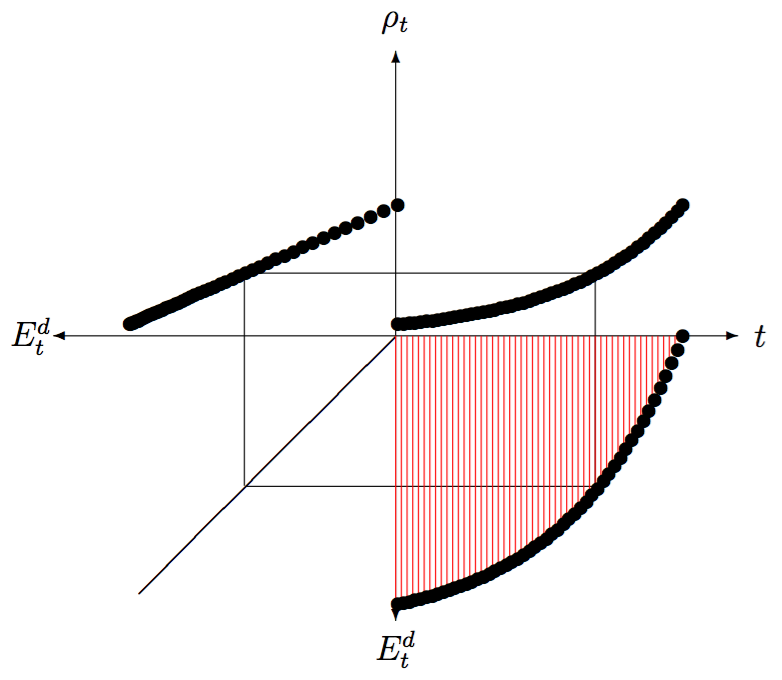
\includegraphics[width=0.5 \linewidth]{hotelling}
\caption{Graphical illustration of Hotelling's rule}
\end{figure}

\paragraph{Marginal rate of substitution (MGRS)}

\begin{align*}
\text{MGRS} := (1+\beta) \frac{u'(c_{t-1})}{u'(c_t)}
\end{align*}

\paragraph{Central planner's problem}

\begin{itemize}
\item With exhaustible resources market equilibria are still Pareto-efficient.
\item The MGRS needs to equal the ratio of marginal productivities of the exhaustible resource:
\begin{align*}
(1+\beta) \frac{u'(c_{t-1})}{u'(c_t)} = \frac{(1+g) \cdot  \partial_e f(k_t,(1+g)^t e_t}{\partial_e f(k_{t-1},(1+g)^{t-1} e_{t-1})}
\end{align*}
\item The MGRS is equal to the marginal productivity minus depreciation:
\begin{align*}
(1+\beta) \frac{u'(c_{t-1}}{u'(c_t)} = \partial_k f(k_t,(1+g)^t e_t) + (1-\kappa)
\end{align*}
\end{itemize}

\paragraph{Market equilibrium}

\begin{itemize}
\item The MGRS is equal to to the risk-free rate:
\begin{align*}
(1+\beta) \frac{u'(c_{t-1}}{u'(c_t)} = 1 + r_t
\end{align*}
\item As expected, the FOC's of the planner's decision problem are equivalent to the the equilibrium conditions of the market equilibrium, i.e. the First Welfare Theorem holds.
\end{itemize}

\subsubsection{Cobb-Douglas production function and logarithmic utility}

\paragraph{Cobb-Douglas production function}

\begin{align*}
Y_t &= K_t^{\alpha_1}((1+g)^t E_t)^{\alpha_2} L_t^{1-\alpha_1-\alpha_2} \\
y_t &= \frac{Y_t}{\bar L_t} = k_t^{\alpha_1}((1+g)^t e_t)^{\alpha_2}
\end{align*}

\begin{itemize}
\item Parameters: $0<\alpha_1,\alpha_2<1$ and $0<\alpha_1+\alpha_2<1$.
\item Variables: $k_t = K_t / \bar L_t$, $e_t = E_t / \bar L_t$.
\end{itemize}

\paragraph{Sustainable technological progress}

\begin{itemize}
\item Parameters (assumed): $g = \beta > n$
\item The rate of technological progress $g = \beta$ allows for a sustainable development of consumption per capita.
\item Extracted exhaustible resources p.c. in period $t$:
\begin{align*}
& e_t = \frac{1}{1-\beta} e_{t-1} = \left( \frac{1}{1-\beta} \right)^t e_0 \\
& \text{with:} \quad e_0 = \frac{\beta-n}{1+\beta} \bar e
\end{align*}
\item The use of exhaustible resources decreases over time.
\item The higher the discount rate $\beta$, the more resources are used by earlier generations.
\item The faster the population grows, the smaller is the level of per capita usage of the exhaustible resource.
\end{itemize}

\paragraph{Technological progress as a growth driver}

\begin{itemize}
\item The extraction of the exhaustible resource is unaffected by technological progress, but decreases with population growth.
\item \emph{Conclusions:} Capital, investment, output and consumption per capita decrease with population growth, but increase with technological progress. \\
In contrast to technological progress, population growth has no impact on growth per capita.
\end{itemize}

\paragraph{Price implications}

\begin{itemize}
\item The growth rate of the prices of exhaustible resources is neither influenced by population growth nor by technological progress for $g = \beta$.
\item The interest rate increases with technological progress, but is unaffected by population growth.
\item Wages are decreasing with population growth but increasing with technological progress.
\end{itemize}

\paragraph{Stock prices}

\begin{itemize}
\item Pricing formula:
\begin{align*}
q_t &= \sum_{\tau=1}^\infty \left( \frac{(1+n)^{1-\alpha} (1+\hat g)^{1-\alpha}}{1+\beta} \right) \pi_t
\end{align*}
\item The real stock price grows with $(1+n)$ and $(1+\hat g)$ over each period.
\item Here, part of the technological progress is needed to offset the effect of a diminishing stock of exhaustible resource and ensure sustainability (hence there is $\hat g$ instead of $g$).
\item Stock prices decline if technological progress is not sufficient to counterbalance the depletion of the exhaustible resource.
\end{itemize}

\subsection{Summary: Population growth and technological progress}

\paragraph{Profits + Population growth}
\begin{itemize}
\item Basic model (Cobb-Douglas production function): increase
\begin{align*}
\pi_n^\ast = (1+n)^\gamma \pi_0^\ast
\end{align*}
\item Basic model + capital (Cobb-Douglas production function with constant returns to scale): constant
\begin{align*}
& \pi^\ast = F(L^\ast,K^\ast) \\
& \qquad - \partial_L F(L^\ast,K^\ast)L^\ast - \partial_K F(L^\ast,K^\ast) K^\ast = 0
\end{align*}
\end{itemize}

\paragraph{Consumption p.c. + Population growth}
\begin{itemize}
\item Basic model with population growth (Cobb-Douglas production function with decreasing returns to scale): decrease
\begin{align*}
c_n^\ast = \frac{C_n^\ast}{\bar L_n} = (1+n)^{\gamma-1} \frac{C_0^\ast}{\bar L_0}
\end{align*}
\item Basic model + capital: decrease \\
(since more people have to produce with the same capital stock they become less productive)
\item Infinite time horizon: constant \\
(since the effect of population growth on the productivity of workers can be counterbalanced by a higher savings rate; a higher savings rate allows keeping the stock of capital p.c. constant)
\item Exhaustible resources: decrease \\
(more workers have to work with the same total amount of exh. resource and thus become less productive; consequently, there is less to consume (unless technological progress advances fast enough))
\end{itemize}

\paragraph{Consumption p.c. + Technological progress}
\begin{itemize}
\item Basic model: increase
\begin{align*}
C_g^\ast = (1+g)^\gamma C_0^\ast
\end{align*}
\item Basic model + capital: increase \\
(more productivity, more can be consumed, more can be invested in the capital stock, which increases consumption in the following periods as well)
\item Infinite time horizon: increase \\
(same reasoning as before; if technology progresses faster than the population grows, then consumption p.c. increases even when the population grows)
\end{itemize}

%\emph{Market equilibria}
%\begin{tabular}{| l | c c c c c |}
%\hline
%Model & Basic Model & Capital & Infinite time horizon & Uncertainty & Exhaustible resources \\
%\hline
%Household's decision problem & $(L^{s\ast},C^\ast) \in \argmax\limits_{L^s,C} U(C)$ \\
%& s.t. $p^\ast C = w^\ast L^s + \pi^\ast, L^s \leq \bar L$ \\
%\hline
%Firm's decision problem & $(L^{d\ast},Y^\ast) \in \argmax\limits_{L^d,Y^\ast} \pi = p^\ast Y - w^\ast L^d$ \\
%\hline
%Market clearing 	& $L^{d\ast} = L^{s\ast}$ \\
%& $C^\ast = Y^\ast$ \\
%\hline
%\end{tabular}

\vfill

\section*{Abbreviations}

\begin{description}[style=multiline,leftmargin=1cm,font=\textbf]
\item[FOC] first order condition
\item[IOT] in order to
\item[p.c.] per capita
\item[RV] random variable
\item[s.t.] such that
\item[w.r.t.] with respect to
\end{description}

\section*{Disclaimer}

\begin{itemize}
\item This summary is work in progress, i.e. neither completeness nor correctness of the content are guaranteed by the author.
\item This summary may be extended or modified at the discretion of the readers.
\item Source: Lecture Economic Foundations for Finance, autumn semester 2015/16, UZH (script, lecture notes and exercises). Copyright of the content is with the lecturers.
\item The layout of this summary is mainly based on the summaries of several courses of the BSc ETH ME from Jonas LIECHTI.
\end{itemize}

\end{multicols*}

\end{document}